\documentclass[a4paper,twoside,12pt,DIV=13,BCOR=5mm,numbers=noenddot,cleardoublepage=empty]{scrbook}
%======= Einbinden der benötigten Packete (= Zusatzfunktionen)
\usepackage[T1]{fontenc}                % für Fonts in westeuropäischer Codierung
\usepackage{lmodern}										% Latin Modern Paket verändert die verwendete Schriftart. Bessere Darstellung für pdf
\usepackage{textcomp}										% Provides extra symbols, e.g. arrows like \textrightarrow, various currencies (\texteuro,..
\usepackage[latin1]{inputenc}    				% german special characters
\usepackage[english,ngerman]{babel}     % hyphenation   usepackage[english,ngerman]{babel} f. deutsch
\usepackage{pdfpages}										% Einbinden von pdf-Files
\usepackage{pifont,textcomp,mathcomp}   % dingbad psfonts and text-compilant fonts (euro, TM, ...)
\usepackage{amsmath,amsopn,amsthm}      % AMS mathematics
\usepackage{amssymb}                    % zusätzliche Symbole 
\usepackage{xspace}											% avoids eaten spaces

%======= Eine Umgebung für Bilder und Tabellen			  	
%\usepackage[textfont={Small},labelfont={bf},margin=1cm,format=plain,font=singlespacing]{caption}   % hanging caption text [hang]
\usepackage[textfont={small},labelfont={bf},margin=1cm,format=plain,font=singlespacing]{caption}   % hanging caption text [hang]
\captionsetup*[figure]{name=Abb.}			 % Abbildungsunterschrift beginnt mit Abb.
\captionsetup*[table]{name=Tab.}


%======= Farben für Überschriften
\usepackage{color}
\definecolor{TUBlau}{rgb}{0,0.4,0.6}   % TU-blau RGB 0 102 153
\addtokomafont{sectioning}{\sffamily\bfseries\selectfont\color{TUBlau}}
\setkomafont{chapter}{\normalfont\huge\sffamily\bfseries\color{TUBlau}}
\addtokomafont{section}{\Large}
\addtokomafont{subsection}{\normalfont\Large\sffamily\bfseries\color{TUBlau}}
\addtokomafont{subsubsection}{\normalfont\large\sffamily\bfseries\color{TUBlau}}
\addtokomafont{paragraph}{\normalfont\large\sffamily\bfseries\color{TUBlau}}


%======= Kopf-/Fußzeilen
\pagestyle{plain} % nur Fußzeile



%======= Eine kompakte Umgebung für die Bilder
\newcommand{\bild}[4]{{
\begin{figure}[#2]
\begin{center}
\includegraphics[scale=#3]{pictures/#1}
\caption{#4}\label{fig:#1}
\end{center}
\end{figure}
}}


%======= Definitionen eigener Befehle
\newcommand{\degC}{\ensuremath{^{\circ}}C}        % Grad Celsius
\newcommand{\Gu}{\glqq{}}                         % Gänsefüßchen unten
\newcommand{\Go}{\grqq{}\xspace}    												% Gänsefüßchen oben











  			% File mit den ben�tigten Packeten, den Formatanweisungen und den Befehlsdefinitionen
\begin{document}

%=============================================================================================
% Titelblatt und Inhaltsverzeichnis
%=============================================================================================
\renewcommand{\baselinestretch}{1.25}
\newcommand{\StudentA}{Karl Mustermann}
\newcommand{\MatrNrA}{10223445}
\newcommand{\StudentB}{Karla Musterfrau}
\newcommand{\MatrNrB}{10223445}
\newcommand{\StudentC}{}
\newcommand{\MatrNrC}{}

\newcommand{\LUDatum}{Unser �bungsdatum}
\newcommand{\LUGruppe}{Unsere Gruppennummer}
\newcommand{\LUBetreuer}{Unser Betreuer}

\large
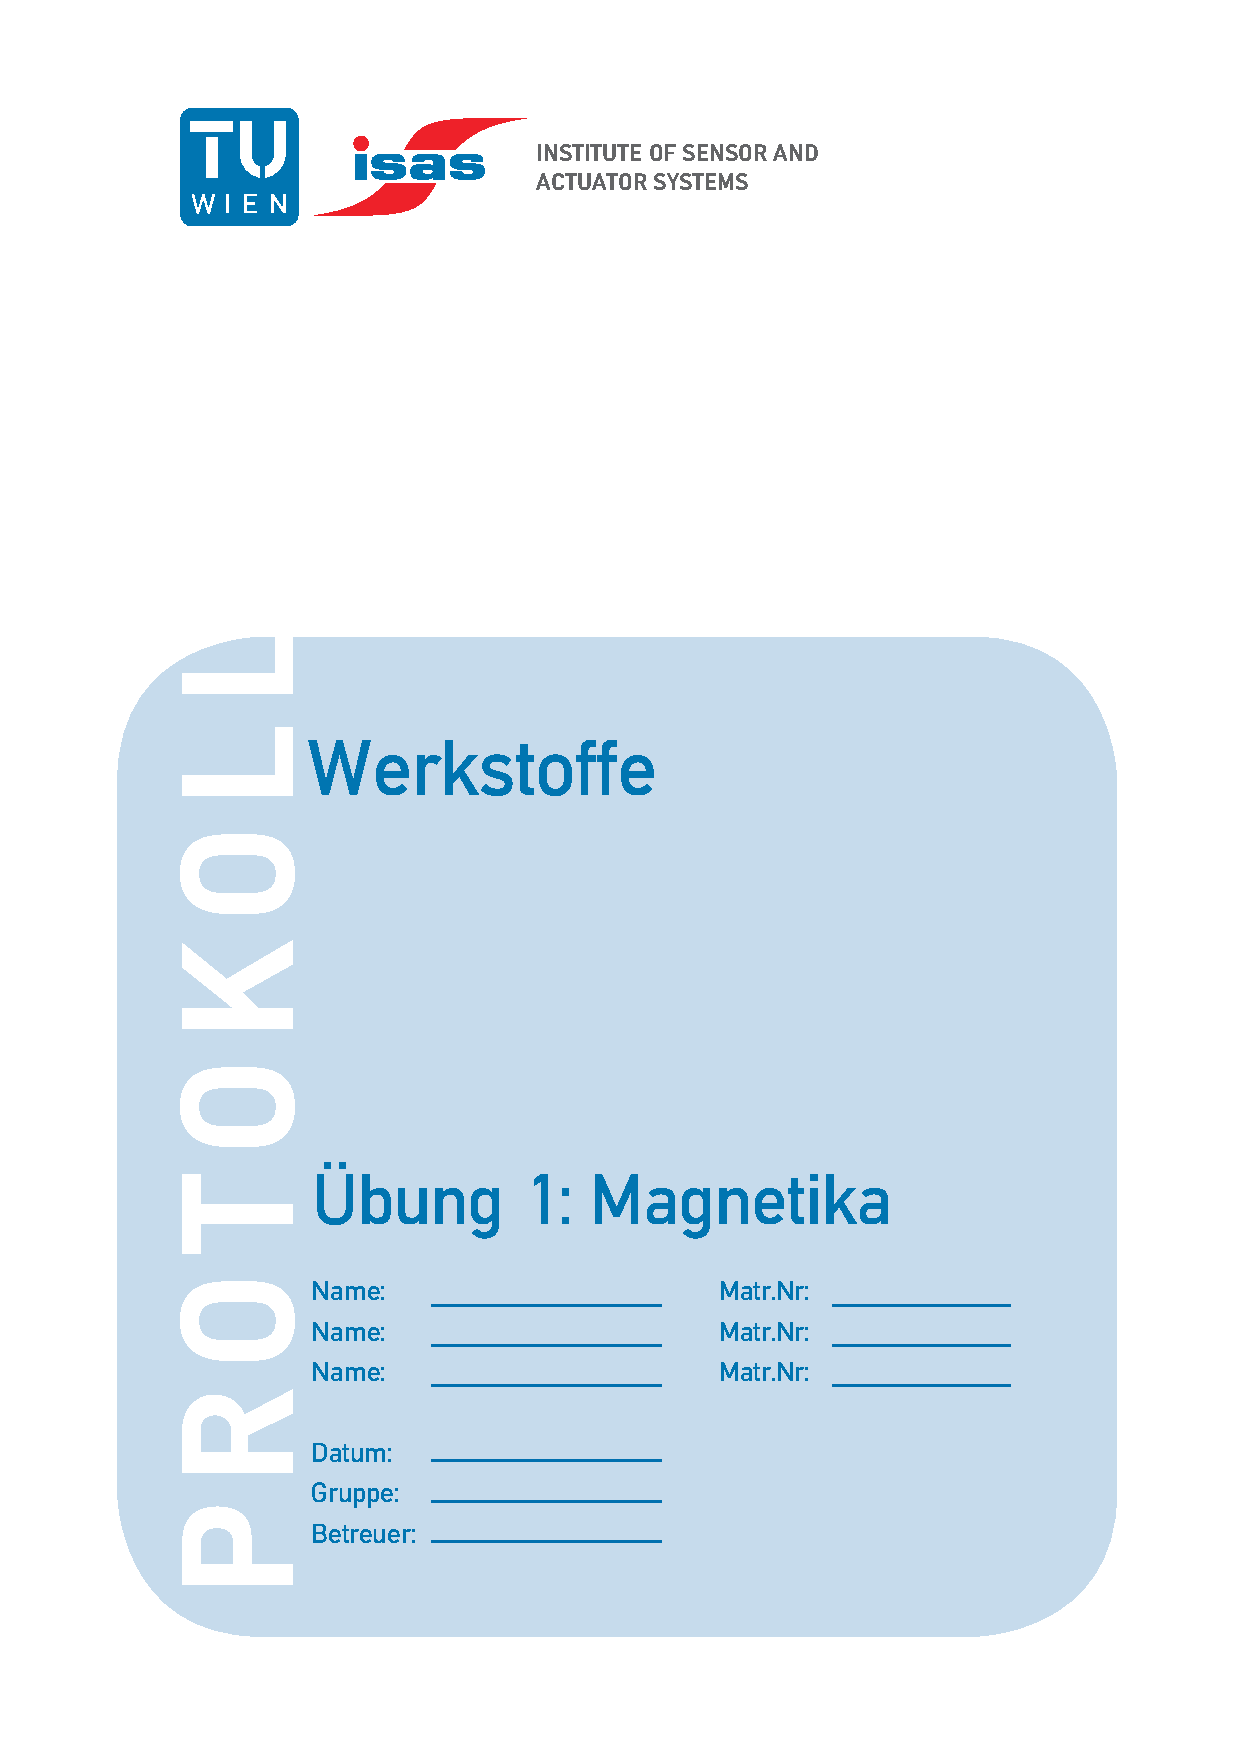
\includepdf[fitpaper=true,
						picturecommand*={\unitlength1cm 
						\put(7.3,7.7){\StudentA} \put(14.1,7.7){\MatrNrA}
            \put(7.3,7.0){\StudentB} \put(14.1,7.0){\MatrNrB}
            \put(7.3,6.3){\StudentC} \put(14.1,6.3){\MatrNrC}
						\put(7.3,5.1){\LUDatum} 
            \put(7.3,4.4){\LUGruppe} 
            \put(7.3,3.7){\LUBetreuer} 
}]
{pictures/DeckblattLUMag}     %file name of title page


%===============================================================================
% Text
%===============================================================================

\cleardoublepage
\setcounter{tocdepth}{3}

\setcounter{page}{0}
\renewcommand{\thepage}{\roman{page}}
\tableofcontents \cleardoublepage

\setcounter{page}{1}
\renewcommand{\thepage}{\arabic{page}}
\setcounter{chapter}{0}


%===============================================================================
\chapter{Einleitung}
%===============================================================================
Dies ist der Beginn einer Unterst�tzung f�r \LaTeX{}-Neulinge, die professionelle technische Dokumente wie Protokolle und Mastarbeiten schreiben wollen. Die erforderliche Software ist Open Source, konstenlos und steht f�r unterschiedlichste Plattformen zur Verf�gung.


%===============================================================================
\chapter{Eine Kapitel�berschrift}
%===============================================================================
Das vorliegende File ist eine minimale \LaTeX{}-Vorlage, wobei Sie das File \Gu ProtokollBeispiel.tex\Go mit einem \LaTeX{}-Editor (z.B. Texniccenter) in ein pdf-File umwandeln m�ssen. 
Sollten Sie noch nie mit \LaTeX{} in Ber�hrung gekommen sein, holen Sie sich am besten Hilfe bei einem Kollegen. Die Installation ist f�r den Anf�nger doch etwas m�hsam und die Art die Texte zu schreiben recht gew�hnungsbed�rftig. Letztendlich lohnt sich der Aufwand wenn gut gesetzte Dokumente mit Formeln und Abbildungen das Ziel sind.  

%-------------------------------------------------------------------------------
\section{Diverses}
%-------------------------------------------------------------------------------
%-------------------------------------------------------------------------------
\subsection{Weiteres}
%-------------------------------------------------------------------------------

Im selben Verzeichnis wie die tex-Datei liegt eine Format-Datei \Gu format-LU.tex\Go in der alle erforderlichen Packages aufgerufen werden und in der auch verschiedene Befehle definiert werden k�nnen (z.\,B. f�r \degC). 

\paragraph{Abbildungen:}
% File wird im Verzeichnis "pictures" gesucht, das unter dem aktuellen Verzeichnis liegt.
% 2. Parameter gibt an, wie Latex das Bild auf der Seite platziert
% 3. Paramter gibt die Skalierung an, am besten Zeichnungen in Orginalgr��er (1.0) erstellen und als pdf einbinden.
% 4. Parameter ist die Bildunterschrift.
\bild{LUKapKopplung1.pdf}{htb}{1.0}{Anordnung zur Messung der kapazitiven Kopplung bei einem Flachbandkabel.}

Legen Sie alle Bilder im Unterverzeichnis \Gu\textbackslash  pictures\Go ab, am Besten im pdf-Format.  
Und hier wird auf die Abbildung Abb.~\ref{fig:LUKapKopplung1.pdf} verwiesen. 


\paragraph{Formeln:}
\begin{equation}
    u_\mathrm{Signal} = G \cdot u_1=10\,\mathrm{V}
\end{equation}

\paragraph{Kinetische Energie (Gleichungsarray):}

\begin{eqnarray*}
    E_{\mathrm{kin}} &=& \frac{m_\mathrm{e} v^2}{2} = \frac{m_\mathrm{e}}{2}\cdot
        \frac{n^2 h^2}{4\pi^2 r^2 m_\mathrm{e}^2}\\
    &=& \frac{m_\mathrm{e}}{2}\cdot
        \frac{n^2 h^2}{4\pi^2 m_\mathrm{e}^2} \cdot
        \frac{\pi^2 e^4 m_\mathrm{e}^2}{\epsilon_0^2 h^4 n^4}\\
    E_{\mathrm{kin}} &=& \frac{1}{2} \cdot \frac{e^4 m_\mathrm{e}}{4 \epsilon_0^2 h^2} \cdot
        \frac{1}{n^2}
\end{eqnarray*}

		\begin{align*}
			\chi &= \varepsilon_\mathrm{r,2} -1 = \frac{N \alpha_\mathrm{OP}}{\varepsilon_0} = N\frac{p^2}{3\varepsilon_0 k_\mathrm{B} T}\\
				 N &= N_\mathrm{A}\cdot\frac{\varrho}{M_\mathrm{H2O}} \\
				   &= \frac{6{,}24\cdot 10^{-30} \cdot 10^6\,\mathrm{g}\cdot \mathrm{mol}}{\mathrm{mol}\cdot\mathrm{m^3}\cdot 18\,\mathrm{g}} = 3{,}3\cdot 10^{28}\,\mathrm{m^{-3}}\\
			   \varepsilon_\mathrm{r,2} &= N\cdot\frac{p^2}{3\varepsilon_0 k_\mathrm{B} T}	+1\\
           &= \frac{3{,}3\cdot 10^{28} \cdot (6{,}24\cdot 10^{-30})^2\,\mathrm{A^2s^2m^2}\cdot \mathrm{Vm} \cdot \mathrm{K}}{\mathrm{m^{-3}} \cdot 3 \cdot 8{,}85\cdot 10^{-12}\,\mathrm{As}\cdot 1{,}38\cdot 10^{-23}\,\mathrm{VAs}\cdot 298\,\mathrm{K}} + 1 = 12{,}8 
		\end{align*}


\paragraph{Eine Liste:}
\begin{itemize}
    \item[$\blacktriangleright$] Element 1
    \item[$\bigstar$] Ein anderes Element und eine kleine Formel $m = 55$\,kg
    \item[$\checkmark$] usw.
\end{itemize}

\noindent Formel im Text kann etwa so geschrieben werden: $H_\mathrm{C} = 12{,}8$\,A/m mit einer Messimpedanz von 10\,M$\Omega \parallel 25$\,pF. Die M�glichkeiten sind beinahe unbeschr�nkt.

\newpage
\bild{LURaster1.pdf}{h!}{0.9}{Kapazitive Kopplung.}

\newpage

%===============================================================================
\chapter{Eine Kapitel�berschrift}
%===============================================================================
Messtemperatur: 25\,\degC, Blechdicke: 25\,\textmu m
%-------------------------------------------------------------------------------
\section{Eine Kapitelunter�berschrift}
%-------------------------------------------------------------------------------


\end{document}


